%\RequirePackage{currfile}
\documentclass[12pt]{beamer}
\usepackage[utf8]{inputenc}
\usepackage[spanish]{babel}
\usepackage{standalone}
\usepackage{color}
\usepackage{siunitx}
\usepackage{hyperref}
\usepackage[outdir=./]{epstopdf}
%\hypersetup{colorlinks,linkcolor=,urlcolor=blue}
%\hypersetup{colorlinks,urlcolor=blue}
\usepackage{xcolor,soul}
\usepackage{etoolbox}
\usepackage{amsmath}
\usepackage{amsthm}
\usepackage{mathtools}
\usepackage{tcolorbox}
\usepackage{physics}
\usepackage{multicol}
\usepackage{bookmark}
\usepackage{longtable}
\usepackage{listings}
\usepackage{cancel}
\usepackage{wrapfig}
\usepackage{empheq}
\usepackage{graphicx}
\usepackage{tikz}
\usetikzlibrary{calc, patterns, matrix, backgrounds, decorations,shapes, arrows.meta}
\usepackage[autostyle,spanish=mexican]{csquotes}
\usepackage[os=win]{menukeys}
\usepackage{pifont}
\usepackage{pbox}
\usepackage{bm}
\usepackage{caption}
\captionsetup{font=scriptsize,labelfont=scriptsize}
%\usepackage[sfdefault]{roboto}  %% Option 'sfdefault' only if the base font of the document is to be sans serif

%Sección de definición de colores
\definecolor{ao}{rgb}{0.0, 0.5, 0.0}
\definecolor{bisque}{rgb}{1.0, 0.89, 0.77}
\definecolor{amber}{rgb}{1.0, 0.75, 0.0}
\definecolor{armygreen}{rgb}{0.29, 0.33, 0.13}
\definecolor{alizarin}{rgb}{0.82, 0.1, 0.26}
\definecolor{cadetblue}{rgb}{0.37, 0.62, 0.63}
\definecolor{deepblue}{rgb}{0,0,0.5}
\definecolor{brown}{rgb}{0.59, 0.29, 0.0}
\definecolor{OliveGreen}{rgb}{0,0.25,0}
\definecolor{mycolor}{rgb}{0.122, 0.435, 0.698}

\newcommand*{\boxcolor}{orange}
\makeatletter
\newcommand{\boxedcolor}[1]{\textcolor{\boxcolor}{%
\tikz[baseline={([yshift=-1ex]current bounding box.center)}] \node [rectangle, minimum width=1ex, thick, rounded corners,draw] {\normalcolor\m@th$\displaystyle#1$};}}
 \makeatother

 \newcommand*\widefbox[1]{\fbox{\hspace{2em}#1\hspace{2em}}}

\newtcbox{\mybox}{on line,
  colframe=mycolor,colback=mycolor!10!white,
  boxrule=0.5pt,arc=4pt,boxsep=0pt,left=6pt,right=6pt,top=6pt,bottom=6pt}

\usefonttheme[onlymath]{serif}
%Sección de definición de nuevos comandos

\newcommand*{\TitleParbox}[1]{\parbox[c]{1.75cm}{\raggedright #1}}%
\newcommand{\python}{\texttt{python}}
\newcommand{\textoazul}[1]{\textcolor{blue}{#1}}
\newcommand{\azulfuerte}[1]{\textcolor{blue}{\textbf{#1}}}
\newcommand{\funcionazul}[1]{\textcolor{blue}{\textbf{\texttt{#1}}}}
\newcommand{\ptilde}[1]{\ensuremath{{#1}^{\prime}}}
\newcommand{\stilde}[1]{\ensuremath{{#1}^{\prime \prime}}}
\newcommand{\ttilde}[1]{\ensuremath{{#1}^{\prime \prime \prime}}}
\newcommand{\ntilde}[2]{\ensuremath{{#1}^{(#2)}}}
\renewcommand{\arraystretch}{1.5}

\newcounter{saveenumi}
\newcommand{\seti}{\setcounter{saveenumi}{\value{enumi}}}
\newcommand{\conti}{\setcounter{enumi}{\value{saveenumi}}}
\renewcommand{\rmdefault}{cmr}% cmr = Computer Modern Roman

\linespread{1.5}

\usefonttheme{professionalfonts}
%\usefonttheme{serif}
\DeclareGraphicsExtensions{.pdf,.png,.jpg}

%Sección para el tema de beamer, con el theme, usercolortheme y sección de footers
\mode<presentation>
{
  \usetheme{Dresden}
  
  %\useoutertheme{infolines}
  \useoutertheme{default}
  \usecolortheme{seahorse}
  \setbeamercovered{invisible}
  % or whatever (possibly just delete it)
  \setbeamertemplate{section in toc}[sections numbered]
  \setbeamertemplate{subsection in toc}[subsections numbered]
  \setbeamertemplate{subsection in toc}{\leavevmode\leftskip=3.2em\rlap{\hskip-2em\inserttocsectionnumber.\inserttocsubsectionnumber}\inserttocsubsection\par}
  \setbeamercolor{section in toc}{fg=blue}
  \setbeamercolor{subsection in toc}{fg=blue}
  \setbeamercolor{frametitle}{fg=blue}
  \setbeamertemplate{caption}[numbered]

  \setbeamertemplate{footline}
  \beamertemplatenavigationsymbolsempty
  \setbeamertemplate{headline}{}
}

\makeatletter
\setbeamercolor{section in foot}{bg=gray!30, fg=black!90!orange}
\setbeamercolor{subsection in foot}{bg=blue!30!yellow, fg=red}
\setbeamertemplate{footline}
{
  \leavevmode%
  \hbox{%
  \begin{beamercolorbox}[wd=.333333\paperwidth,ht=2.25ex,dp=1ex,center]{section in foot}%
    \usebeamerfont{section in foot} \insertsection
  \end{beamercolorbox}}%
  \begin{beamercolorbox}[wd=.333333\paperwidth,ht=2.25ex,dp=1ex,center]{subsection in foot}%
    \usebeamerfont{subsection in foot}  \insertsubsection
  \end{beamercolorbox}%
  \begin{beamercolorbox}[wd=.333333\paperwidth,ht=2.25ex,dp=1ex,right]{date in head/foot}%
    \usebeamerfont{date in head/foot} \insertshortdate{} \hspace*{2em}
    \insertframenumber{} / \inserttotalframenumber \hspace*{2ex} 
  \end{beamercolorbox}}%
  \vskip0pt%
\makeatother  

\makeatletter
\patchcmd{\beamer@sectionintoc}
  {\vfill}
  {\vskip\itemsep}
  {}
  {}
\makeatother


\title{\large{Polinomios de Legendre}}
\subtitle{Construcción alterna}
\author{M. en C. Gustavo Contreras Mayén}
\date{}
\institute{Facultad de Ciencias - UNAM}
\titlegraphic{
\includegraphics[width=1.75cm]{../Imagenes/escudo-facultad-ciencias}\hspace*{4.75cm}~%
   
\includegraphics[width=1.75cm]{../Imagenes/escudo-unam}
}
\setbeamertemplate{navigation symbols}{}
\begin{document}
\maketitle
\fontsize{14}{14}\selectfont
\spanishdecimal{.}
\section*{Contenido}
\frame[allowframebreaks]{\tableofcontents[currentsection, hideallsubsections]}
\section{Polinomios de Legendre}
\frame{\tableofcontents[currentsection, hideothersubsections]}
\subsection{Introducción}
\begin{frame}
\frametitle{Funciones especiales}
A partir de este tema abordaremos las \emph{funciones especiales}.
\\
\bigskip
\pause
Una propiedad fundamental de estas funciones, es que todas ellas son soluciones a uno o más problemas de la física.
\end{frame}
\begin{frame}
\frametitle{Función generadora}
Parten a su vez, de una función generadora, es decir, es posible construir una función $g(x, t)$ que contiene la información de toda la familia de funciones.
\end{frame}
\begin{frame}
\frametitle{Función generadora}
Los miembros de una familia de funciones poseen relaciones entre miembros de orden superior y entre sus derivadas.
\\
\bigskip
\pause
Al conjuntar estos elementos, se muestra que estas familias de funciones son soluciones a una ED2 que modela un problema de la física.
\end{frame}
\begin{frame}
\frametitle{Pilar del curso}
Esta relación cíclica es uno de los pilares de este curso, veremos la construcción de los polinomios de Legendre como una herramienta de estudio para el \emph{desarrollo multipolar eléctrico}.
\\
\bigskip
\pause
Y como se ha estado revisando, los polinomios de Legendre forman parte de la solución angular del átomo de hidrógeno.
\end{frame}
\section{Desarrollo multipolar}
\frame{\tableofcontents[currentsection, hideothersubsections]}
\subsection{Construcción geométrica}
\begin{frame}
\frametitle{Construcción}
Consideremos un sistema de $N$ cargas puntuales
\begin{align*}
\left\{ q_{i} \, | \, 1 \leq i \leq N \right\}
\end{align*}
localizadas en un volumen $V$.
\end{frame}
\begin{frame}
\frametitle{Descripción geométrica}
\begin{figure}
    \centering
    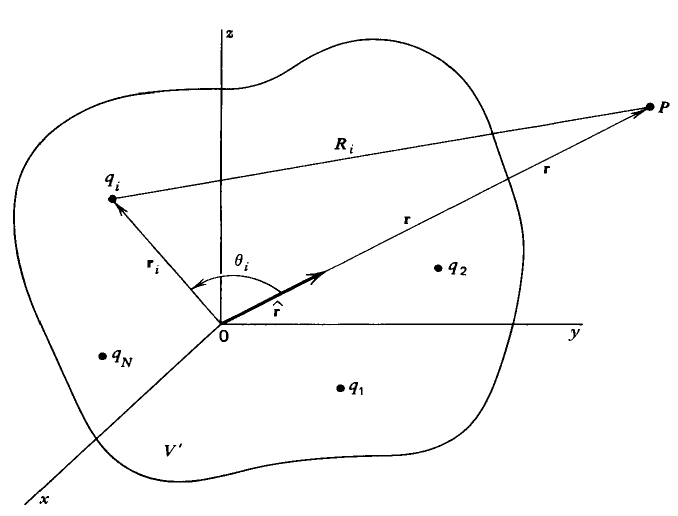
\includegraphics[scale=0.3, keepaspectratio]{Imagenes/Desarrollo_multipolar.png}
    \caption{Geometría para el cálculo del potencial debido a un sistema de cargas puntuales.}
    \label{fig:figura_multipolar_01}
\end{figure}
\end{frame}
\begin{frame}
\frametitle{Construcción}
Se toma como origen $O$ de coordenadas un punto arbitrario pero conveniente, que se encuentre ya sea en $V$ o cercá de éste.
\\
\bigskip
\pause
Los vectores de posición de las cargas son
\begin{align*}
\vb{r}_{1}, \vb{r}_{2}, \ldots, \vb{r}_{N}  
\end{align*}
\end{frame}
\begin{frame}
\frametitle{Problema}
Se desea obtener el potencial $\phi$, en el punto de campo $P$, cuyo vector de posición con respecto a este mismo origen es $\vb{r}$.
\\
\bigskip
\pause
Por lo que $P$ se encuentra en la dirección $\hat{\vb{r}}$ a una distancia $r$ de $O$.
\end{frame}
\begin{frame}
\frametitle{El potencial}
Este potencial está dado como
\begin{align}
\phi(\vb{r}) = \sum_{i=1}^{N} \dfrac{q_{i}}{4 \,\pi \, \varepsilon_{0} \, R_{i}}
\label{eq:ecuacion_08_01}
\end{align}
donde $R_{i} = \abs{\vb{r} - \vb{r}_{i}}$
\end{frame}
\begin{frame}
\frametitle{Uso del ángulo}
Si ocupamos el ángulo $\theta_{i}$ entre las direcciones de $\vb{r}_{i}$ y $\vb{r}$ y ocupando la ley de los cosenos, de la figura (\ref{fig:figura_multipolar_01}), tendremos que:
\begin{align}
R_{i} = \big( r^{2} + r_{i}^{2} - 2 \, r \, r_{i} \, \cos \theta_{i} \big)^{1/2}
\label{eq:ecuacion_08_02}
\end{align}
\end{frame}
\begin{frame}
\frametitle{Expresión para el potencial}
Por lo que la ec. (\ref{eq:ecuacion_08_01}) queda como:
\begin{align}
\phi(\vb{r}) = \sum_{i=1}^{N} \dfrac{q_{i}}{4 \,\pi \, \varepsilon_{0} \, \big( r^{2} + r_{i}^{2} - 2 \, r \, r_{i} \, \cos \theta_{i} \big)^{1/2}}
\label{eq:ecuacion_08_03}
\end{align}
\end{frame}
\begin{frame}
\frametitle{Primera pausa}
No podemos hacer algo más a menos que conozcamos los detalles exactos de la distrubución de las cargas.
\\
\bigskip
\pause
Supongamos que el punto $P$ está lo suficientemente alejado de $V$ de está más lejos del origen que cualquiera de las cargas.
\end{frame}
\begin{frame}
\frametitle{Avance}
En esta suposición, tendremos que $r > \vb{r}_{i}$ para toda $i$, entonces la relación $(r_{i}/r)$ es siempre menor que uno, por lo que podemos considerar un desarrollo en serie de potencias de esta relación.
\end{frame}
\begin{frame}
\frametitle{Avance}
Si se factoriza la $r^{2}$ de la raíz cuadrada de la ec. (\ref{eq:ecuacion_08_02}), podremos escribir
\begin{align}
\dfrac{1}{R_{i}} = \dfrac{1}{r (1 + t)^{1/2}}
\label{eq:ecuacion_08_04}
\end{align}
\pause
donde
\begin{align}
t = -2 \left( \dfrac{r_{i}}{r} \right) \, \cos \theta + \left( \dfrac{r_{i}}{r} \right)^{2}
\label{eq:ecuacion_08_05}
\end{align}
\end{frame}
\begin{frame}
\frametitle{Desarrollando la serie de potencias}
Ahora podemos usar la serie de potencias:
\begin{align}
(1 \pm t)^{-(1/2)} = 1 \mp \dfrac{1}{2} \, t + \dfrac{3}{8} \, t^{2} \mp \dfrac{5}{16} t^{3} + \ldots
\label{ec:ecuacion_08_06}
\end{align}
con el signo superior, para desarrollar la raíz cuadrada en la ec. (\ref{eq:ecuacion_08_04})
\end{frame}
\begin{frame}
\frametitle{Términos de orden cuadrático}
Se mantienen todos los términos del orden de $(r_{i}/r)^{2}$ y omitimos el resto, ya que no será necesario utilizar el cuarto término del desarrollo que incluye a $t^{3}$, y por lo tanto a $(r_{i}/r)^{3}$.
\end{frame}
\begin{frame}
\frametitle{Términos de orden cuádratico}
Al sustituir la ec. (\ref{eq:ecuacion_08_05}) en la ec. (\ref{ec:ecuacion_08_06}) y omitiendo los términos que contienen a $(r_{i}/r)^{3}$ y $(r_{i}/r)^{4}$, tendremos que:
\end{frame}
\begin{frame}
\frametitle{Términos de la serie}
\begin{eqnarray*}
\dfrac{1}{(1 + t)^{1/2}} &\simeq& 1 - \dfrac{1}{2} \left[ -2 \left( \dfrac{r_{i}}{r} \right) \, \cos \theta_{i} + \left( \dfrac{r_{i}}{r} \right)^{2} \right] + \\[0.5em]
&+& \dfrac{3}{8} \left[ -2 \left( \dfrac{r_{i}}{r} \right) \, \cos \theta_{i} + \left( \dfrac{r_{i}}{r} \right)^{2} \right]^{2} \\[0.5em] \pause
&\simeq& 1 {+} \left( \dfrac{r_{i}}{r} \right) \cos \theta_{i} {+} \dfrac{1}{2} \left( \dfrac{r_{i}}{r} \right)^{2} \, (3 \, \cos \theta_{i} - 1)
\end{eqnarray*}
\end{frame}
\begin{frame}
\frametitle{El potencial obtenido}
Al dividir la expresión anterior entre $r$, y de acuerdo con la ec. (\ref{eq:ecuacion_08_04}), al sustituir el resultado en la ec. (\ref{eq:ecuacion_08_01}), tendremos que el potencial estará dado por la expresión:
\end{frame}
\begin{frame}
\frametitle{El potencial obtenido}
\begin{align}
\begin{aligned}[b]
\phi(\vb{r}) &= \dfrac{1}{4 \pi \varepsilon_{0} r} \sum_{i=1}^{N} q_{i} + \dfrac{1}{4 \pi \varepsilon_{0} r^{2}} \sum_{i=1}^{N} q_{i} \, r_{i} \, \cos \theta_{i} + \\[0.5em]
&+ \dfrac{1}{4 \pi \varepsilon_{0} r^{3}} \sum_{i=1}^{N} \dfrac{q_{i} \, r_{i}^{2}}{2} (3 \, \cos^{2} \theta_{i} - 1) + \ldots
\end{aligned}
\label{eq:ecuacion_08_07}
\end{align}
\pause
Es claro que hay más términos en el desarrollo pero éstos no se ha calculado.
\end{frame}
\begin{frame}
\frametitle{Los términos}
Los términos individuales de la suma se llama, respectivamente, el término monopolar, el término dipolar, el término cuadripolar.
\\
\bigskip
\pause
Vemos que mantienen una dependencia con la distancia $r$ del punto de campo, de la forma $1/r$, $1/r^{2}$, $1/r^{3}$, etc., a medida de que se van alejando de la distribución de carga, los términos de mayor orden son cada vez menos importantes.
\end{frame}
\begin{frame}
\frametitle{El potencial}
De manera conveniente, el potencial obtenido se expresa como:
\begin{align}
\phi(\vb{r}) = \phi_{M}(\vb{r}) + \phi_{D}(\vb{r}) + \phi_{Q}(\vb{r}) + \ldots
\label{eq:ecuacion_08_08}
\end{align}
\end{frame}
\section{Abordaje matemático}
\frame{\tableofcontents[currentsection, hideothersubsections]}
\subsection{Polinomios de Legendre}
\begin{frame}
\frametitle{Serie polinomial}
Dejando a un lado el contexto físico y entrando a un estudio matemático, notemos que la función:
\begin{align*}
\dfrac{1}{\left( 1 + \left( \dfrac{r_{i}}{r} \right)^{2} + 2 \left( \dfrac{r_{i}}{r} \right) \, \cos \theta_{i} \right)^{1/2}}
\end{align*}
genera una serie polinomial en el $\cos \theta_{i}$.
\end{frame}
\begin{frame}
\frametitle{Cambio de variable}
Ahora sean $x$ e $y$, tales que:
\begin{align*}
x = \cos \theta_{i} \hspace{1.5cm} y = \left( \dfrac{r_{i}}{r} \right)
\end{align*}
entonces:
\pause
\begin{align*}
\dfrac{1}{(1 + y^{2} - 2 \, y \, x)^{1/2}} = \sum_{\ell=0}^{\infty} P_{\ell} (x) \, y^{\ell}
\end{align*}
tal que $\abs{x} \leq 1$, $y < 1$
\end{frame}
\begin{frame}
\frametitle{Polinomios de Legendre}
Tal que las siguientes expresiones:
\begin{eqnarray*}
P_{0} (x) &=& 1 \\[0.5em] \pause
P_{1} (x) &=& x \\[0.5em] \pause
P_{2} (x) &=& \dfrac{1}{2} (3 \, x^{2} - 1) \\
\vdots
\end{eqnarray*}
\pause
Se conocen como los \emph{Polinomios de Legendre}.
\end{frame}
\begin{frame}
\frametitle{Siguiente paso}
El siguiente paso es: determinar la representación del n-ésimo polinomio de Legendre, así como procedimientos alternativos para construirlos.
\end{frame}
\begin{frame}
\frametitle{Regresando al potencial}
Obtuvimos que el potencial multipolar está dado por:
\begin{eqnarray*}
\phi(\vb{r}) &=& \dfrac{1}{4 \pi \varepsilon_{0} r} \sum_{i=1}^{N} \dfrac{q_{i}}{\left[ 1 + \left( \dfrac{r_{i}}{r} \right)^{2} + 2 \left( \dfrac{r_{i}}{r} \right) \, \cos \theta_{i} \right]^{1/2}} = \\[0.5em] \pause
&=& \dfrac{1}{4 \pi \varepsilon_{0} r} \sum_{i=1}^{N} q_{i} \sum_{\ell=0} \left( \dfrac{r_{i}}{r} \right)^{\ell} \, P_{\ell} (\cos \theta) =
\end{eqnarray*}
\end{frame}
\begin{frame}
\frametitle{Regresando al potencial}
Para cada carga $i$:
\begin{align*}
\phi_{i} (\vb{r}) = \dfrac{q_{i}}{4 \pi \varepsilon_{0} r} \sum_{\ell=0}^{N} \left( \dfrac{r_{i}}{r} \right)^{\ell} \, P_{\ell} (\cos \theta)
\end{align*}
\end{frame}
\begin{frame}
\frametitle{Representación de los polinomios}
De la expresión:
\begin{align*}
\phi(\vb{r}) = \dfrac{q}{4 \pi \varepsilon_{0} (r^{2} + r_{i}^{2} - 2 r \, r_{i} \, \cos \theta)^{1/2}}
\end{align*}
\pause
asumiremos que $\abs{r_{i}} = a$, por lo que el potencial eléctrico está dado por:
\end{frame}
\begin{frame}
\frametitle{Potencial eléctrico}
\begin{eqnarray*}
\phi(\vb{r}) &=& \dfrac{q}{4 \pi \varepsilon_{0} \, r \left[ 1 + \left( \dfrac{a}{r} \right)^{2} - 2 \left( \dfrac{a}{r} \right) \, \cos \theta \right]^{1/2}} \\[0.5em] \pause
&=& \dfrac{q}{4 \pi \varepsilon_{0} \, r} \sum_{\ell=0}^{\infty} \left( \dfrac{a}{r} \right)^{\ell} \, P_{\ell} (\cos \theta)
\end{eqnarray*}
\end{frame}
\begin{frame}
\frametitle{Resultado equivalente}
Entonces tendremos que:
\begin{align*}
\dfrac{1}{\left[ 1 + \left( \dfrac{a}{r} \right)^{2} - 2 \left( \dfrac{a}{r} \right) \, \cos \theta \right]^{1/2}} = \sum_{\ell=0}^{\infty} \left( \dfrac{a}{r} \right)^{\ell} \, P_{\ell} (\cos \theta)
\end{align*}
\end{frame}
\subsection{Función generatriz}
\begin{frame}
\frametitle{Función generatriz}
A la función:
\begin{align*}
\dfrac{1}{\left[ 1 + \left( \dfrac{a}{r} \right)^{2} - 2 \left( \dfrac{a}{r} \right) \, \cos \theta \right]^{1/2}}
\end{align*}
cuya expansión en una serie de Taylor, construye los polinomios de Legendre, se le conoce como \emph{función generadora (o generatriz)}.
\end{frame}
\begin{frame}
\frametitle{Función generatriz}
Sea $x = \cos \theta$, y $t = (a/r)$, entonces:
\begin{align*}
g(x, t) = \dfrac{1}{\left[ 1 + t^{2} - 2 \, t \, x \right]^{1/2} } = \sum_{\ell=0}^{\infty} t^{\ell} \, P_{\ell} (x)
\end{align*}
\pause
Nos fijamos ahora en el denominador del lado izquierdo, para revisar si se puede expandir en una serie de Taylor.
\end{frame}
\begin{frame}
\frametitle{Expasión en Taylor}
Definimos $z = t^{2} - 2 \, t \, x$ con $\abs{z} < 1$, por lo que
\begin{align*}
(1 + z)^{1/2}
\end{align*}
puede ser expandido en una serie de Taylor: 
\pause
\fontsize{12}{12}\selectfont
\begin{align*}
(1 + z)^{1/2} = \dfrac{f(0)}{0!} - \dfrac{\ptilde{f}(0) \, z}{1!} + \dfrac{\stilde{f}(0) \, z^{2}}{2!} - \dfrac{\ttilde{f}(0) \, z^{3}}{3!} + \ldots
\end{align*}
\end{frame}
\begin{frame}
\frametitle{Expansión en Taylor}
Haciendo el álgebra correspondiente, tendremos que:
\begin{align*}
(1 + z)^{1/2} = \sum_{n=0}^{\infty} \dfrac{(-1)^{n} \, (2 n)!}{2^{2 n} \, [n!]} \, \dfrac{z^{n}}{n!}
\end{align*}
\pause
Por lo que la función generatriz:
\end{frame}
\begin{frame}
\frametitle{La función generatriz}
La función generatriz se expresa:
\begin{eqnarray*}
g(x, z) &=& \sum_{n=0}^{\infty} \dfrac{(-1)^{n} \, (2 n)!}{2^{2 n} \, [n!]^{2}} z^{n} = \\[0.5em] \pause
&=& \sum_{\ell=0}^{\infty} \dfrac{(-1)^{\ell} \, (2 \ell)!}{2^{2 \ell} \, [\ell!]^{2}} z^{\ell} = \\[0.5em] \pause
&=& \sum_{\ell=0}^{\infty} \dfrac{(-1)^{\ell} \, (2 \ell)!}{2^{2 \ell} \, [\ell!]^{2}} (t^{2} - 2 \, t \, x)^{\ell} = 
\end{eqnarray*}
\end{frame}
\begin{frame}
\frametitle{La función generatriz}
\begin{eqnarray*}
g(x, z) &=& \sum_{\ell=0}^{\infty} \dfrac{(-1)^{\ell} \, (2 \ell)! \, t^{\ell}}{2^{2 \ell} \, [\ell!]^{2}} (t - 2 \, x)^{\ell} = \\[0.5em] \pause
&=& \sum_{\ell=0}^{\infty} \dfrac{(-1)^{\ell} \, (2 \ell)! \, t^{\ell}}{2^{2 \ell} \, [\ell!]^{2}} \sum_{k=0}^{\ell} \binom{\ell}{k} \, t^{k} (-2 \, k)^{\ell - k}
\end{eqnarray*}
\end{frame}
\begin{frame}
\frametitle{Haciendo el álgebra}
\begin{eqnarray*}
g(x, z) &=& \sum_{\ell=0}^{\infty} \, \sum_{k=0}^{\ell} \dfrac{(-1)^{k} \, (2 \ell)! \, \, (2 \, x)^{\ell -k} \, t^{\ell+k}}{2^{2 \ell} \, \ell! \, k! \, (\ell - k)!} = \\[0.5em] \pause
&=& \sum_{\ell=0}^{\infty} \, \sum_{k=0}^{[\frac{\ell}{2}]} \dfrac{(-1)^{k} \, (2 \ell - 2 k)! \, (2 \, x)^{\ell -k} \, t^{\ell}}{2^{2 \ell - 2 k} \, (\ell - k)! \, k! \, (\ell - 2 \, k)!}
\end{eqnarray*}
\end{frame}
\begin{frame}
\frametitle{Los polinomios de Legendre}
\begin{align*}
P_{\ell} (x) = \sum_{k=0}^{[\frac{\ell}{2}]} \dfrac{(-1)^{k} \, (2 \ell - 2 k)! \, (2 \, x)^{\ell -k} \, t^{\ell}}{2^{2 \ell - 2 k} \, (\ell - k)! \, k! \, (\ell - 2 \, k)!}
\end{align*}
\pause
Hasta este punto conocemos los polinomios de Legendre, sin embargo nos interesa obtener un procedimiento más versátil que nos permita calcular los $P_{\ell}(x)$.
\end{frame}
\end{document}